\section{Concept}
\label{sec:concept}

As mentioned in section \ref{sec:intro}, data produced by sensors on wearables needs to be transferred to mobile devices in order to be processed.
All Android Wear devices are connected via Bluetooth, we will use this connection to exhange the data with the mobile device.

\begin{figure}[H]
	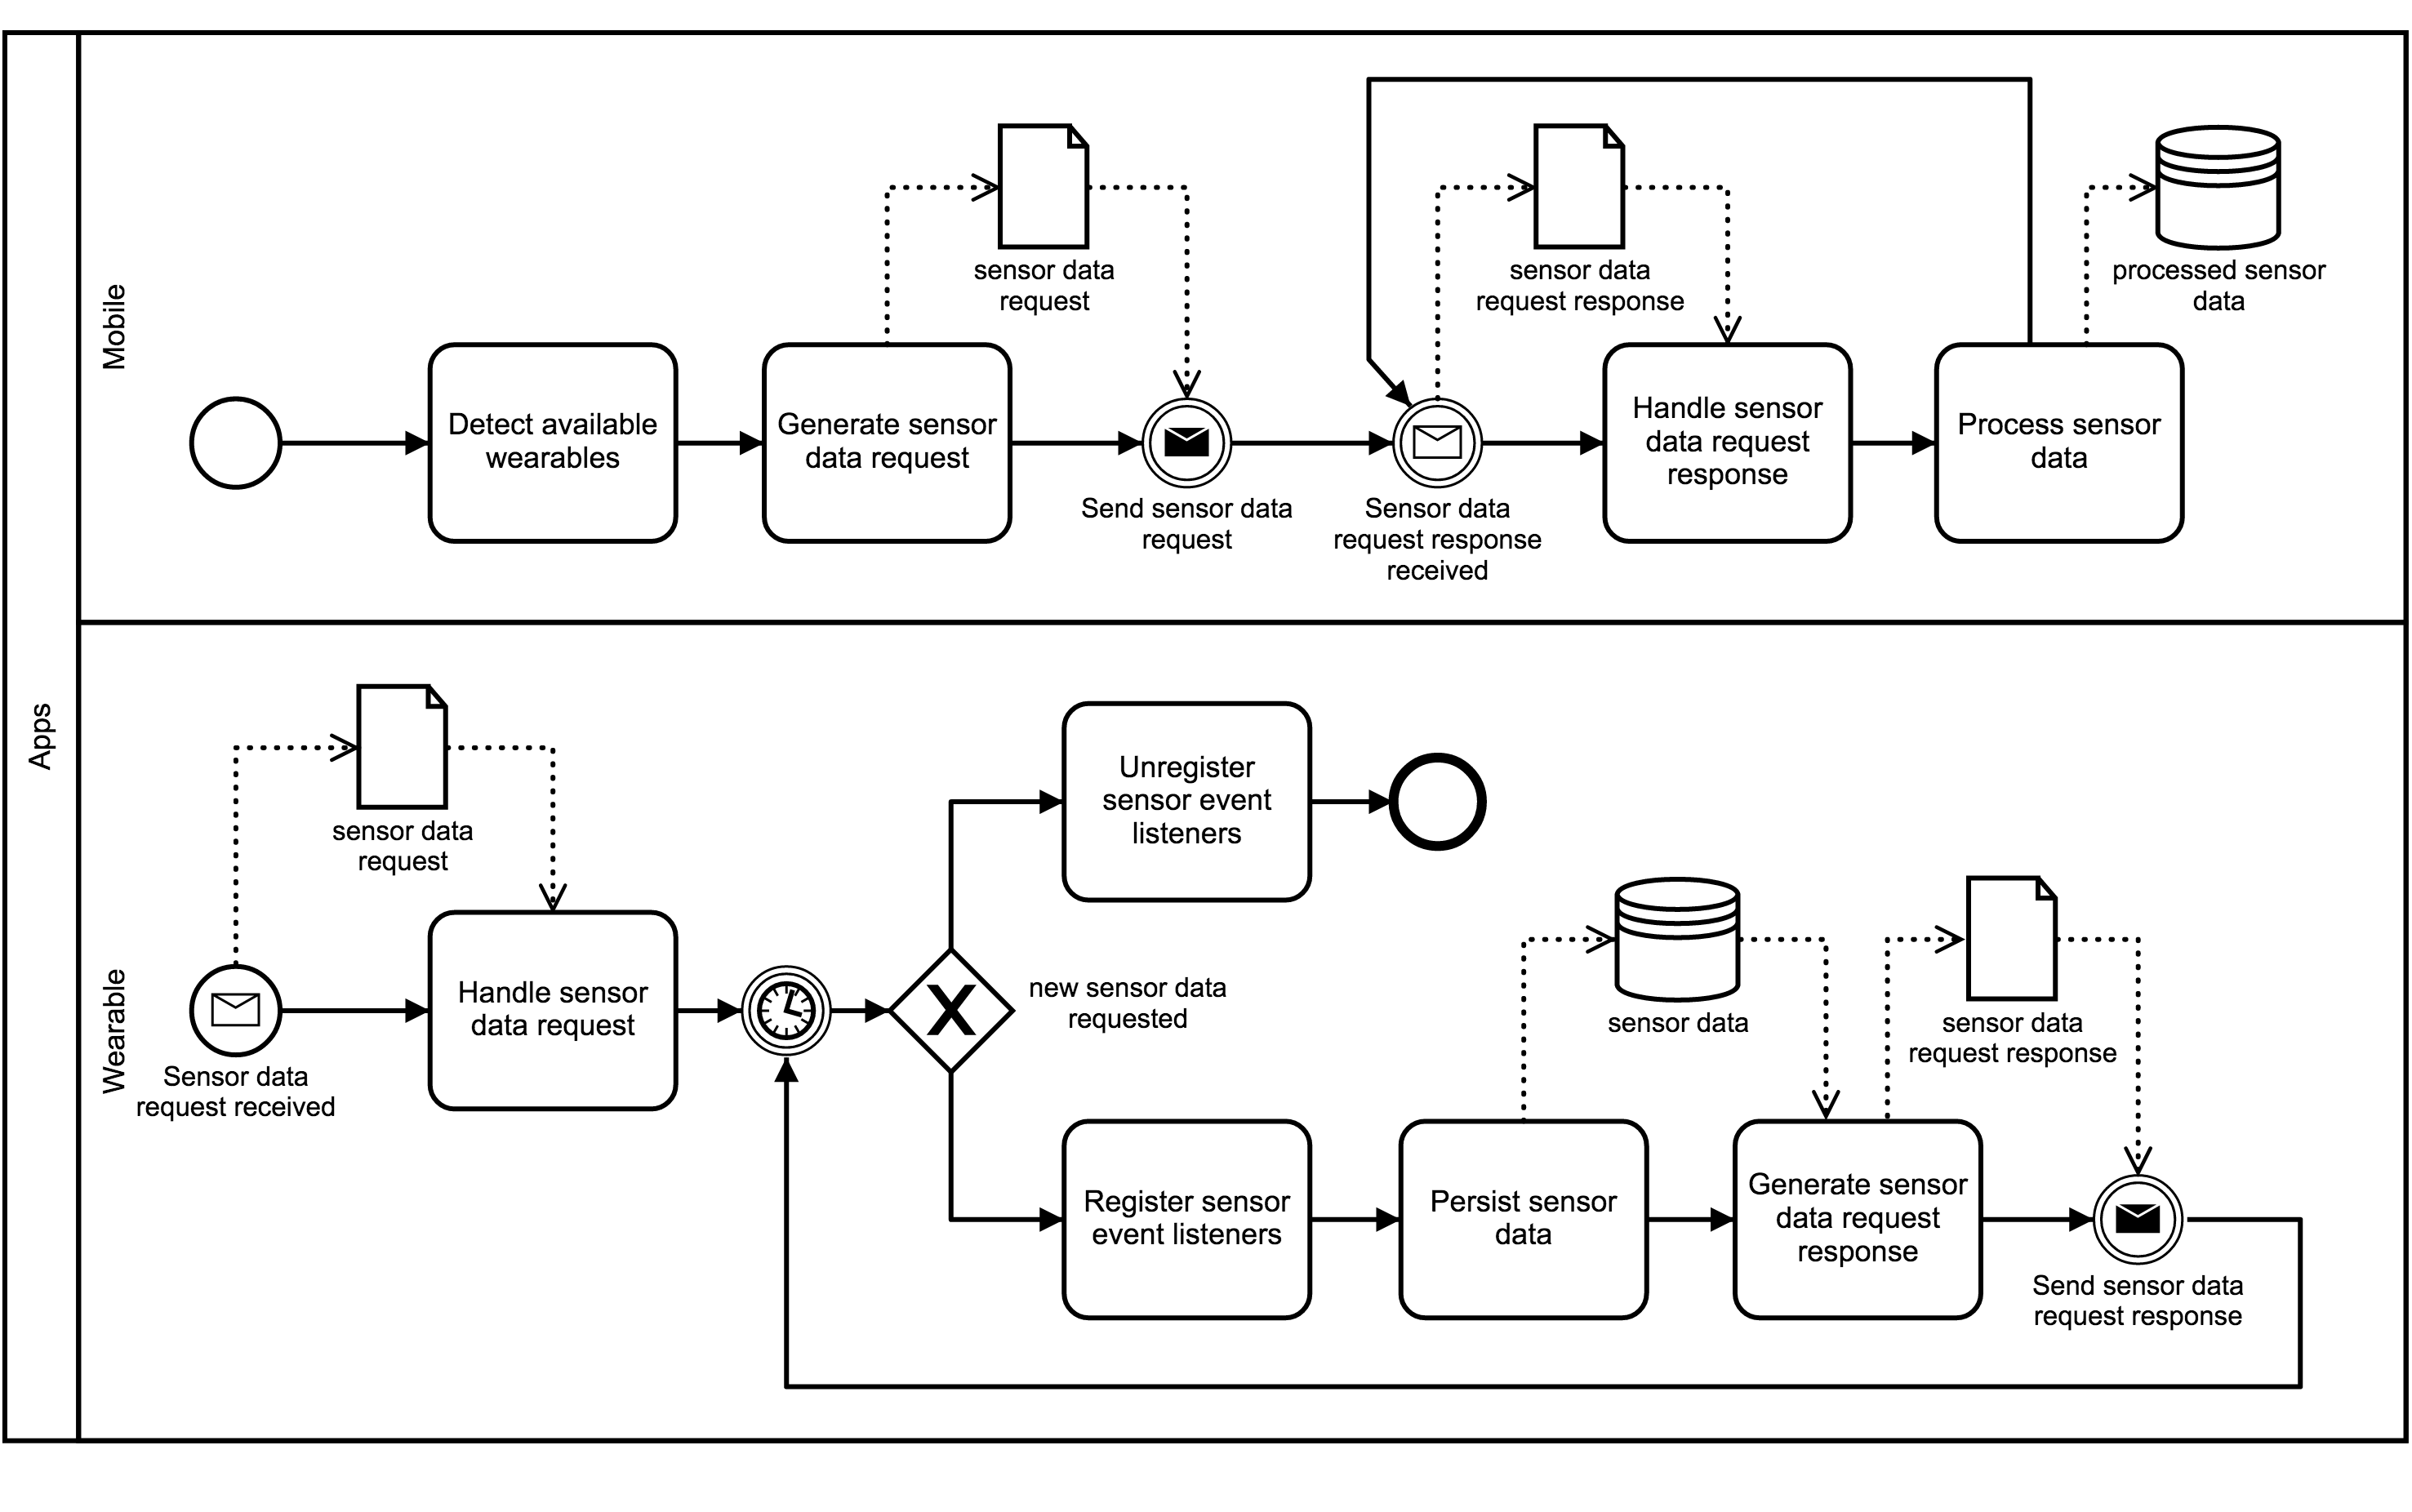
\includegraphics[width=\linewidth]{diagrams/apps.png}
	\caption[Caption for bpmn]{App process model}
	\label{fig:diagrams:apps}
\end{figure}

In order to fulfill the requirements mentioned in section \ref{sec:intro:scope}, we need two different apps to be deployed.
One on the mobile device, another one on each wearable device.
Figure \ref{fig:diagrams:apps} shows what both apps need to be capable of.

\clearpage

\subsection{Mobile App}
\label{sec:concept:mobileapp}
The app deployed on the mobile device is responsible of:
\begin{itemize}[noitemsep]
	\item Sending sensor data requests
	\item Handling sensor data request responses
	\item Processing received sensor data
\end{itemize}

Once started, it sends a sensor data request to connected wearable devices, which contains information about which sensor data it wants to receive and at which interval (see section \ref{sec:implementation:transferringdata:send}).
The app then listens for incoming sensor data request responses, which contain the actual sensor data (see section \ref{sec:implementation:transferringdata:receive}).
This data will be processed depending on the use case.

\subsection{Wearable App}
\label{sec:concept:wearableapp}
The wearable app on the other side takes care of:
\begin{itemize}[noitemsep]
	\item Handling sensor data requests
	\item Accessing and persisting sensor data
	\item Sending sensor data request responses
\end{itemize}

After deployment, it waits for incoming sensor data requests.
It registers the required sensor listeners and starts monitoring data changes (see section \ref{sec:implementation:monitoringdatachanges}).
Updated sensor data request responses will be periodically sent to the mobile app until the sensor data request changes.

\clearpage